\documentclass[tikz]{standalone} % border={left bottom right top}
\usepackage{tikz}
\usepackage{tikz-3dplot}
\usetikzlibrary{shadings,decorations.markings,arrows.meta,quotes,angles,snakes,decorations}
\usepackage{xcolor}
\usepackage{amsmath}
\usepackage{marvosym}

\tikzset{
    %Define standard arrow tip
    >=stealth'
}

\tikzset{
    tst/.style={
      thin, opacity=0.5,
      dashed
    },
    my-arc/.style={
      start angle=0, end angle=360,radius=0.4
    }
}

\tikzset{
    ->-/.style={
        decoration={markings, mark=at position #1 with {\arrow{>}}},
        postaction={decorate}
    },
    scatter/.style={decorate, draw=black,
        decoration={complete sines,amplitude=8pt, segment length=11pt}}
}

\definecolor{blue}{RGB}{92, 96,176}
\definecolor{red}{RGB}{223, 99,140}
\definecolor{green}{RGB}{83,192,97}
\definecolor{yellow}{RGB}{253,216,112}
\definecolor{gray}{RGB}{109,109,109}
\definecolor{lightgray}{RGB}{200,200,200}
\definecolor{orange}{RGB}{239,142,79}

% \newcommand{\bbox}[1]{%
%   \color{red!50}\rlap{\fbox{$\phantom{#1}$}}%
%   \color{black}#1%
% }

\def\cTens#1#2#3 {
    \begin{scope}[shift={#3}]
        	\fill[#1] (0,0) circle (#2);
        	\clip (0,0) circle (#2);
	\shade[outer color=#1, inner color=#1!70] (-#2,#2) circle (1.75*#2);
	\draw[very thin] (0,0) circle (#2);
		\end{scope}
}

\def\rTens#1#2#3#4 {
	\begin{scope}[shift={#4}]
	        	\fill[#1] (-#2/2,-#3/2) rectangle (#2/2,#3/2);
	        	\clip (-#2/2,-#3/2) rectangle (#2/2,#3/2);
		\shade[outer color=#1, inner color=#1!70] (-1.41*#2/2,1.41*#3/2)  circle (1.3*#3/2+1.3*#2/2);
		\draw[very thin] (-#2/2,-#3/2) rectangle (#2/2,#3/2);
	\end{scope}
}

\def\oTens#1#2#3 {
    \begin{scope}[shift={#3}]
        	\fill[#1] (0,0) circle (#2);
        	\clip (0,0) circle (#2);
	\shade[outer color=#1, inner color=#1!70] (-#2,#2) circle (1.75*#2);
	\draw[very thin] (0,0) circle (#2);
		\end{scope}
}

%!TEX root = thesis.tex
%%%%%%%%%%%%%%%%%%%%%
\def\ri{\mathrm i}
\def\re{\mathrm e}
\def\rd{\mathrm d}
\def\rD{\mathcal D}
\def\hc{{\rm h.c.}}
\def\tr{{\rm tr}}
\def\C{\mathcal{C}}
\def\DC{\Delta\C}
\def\GX{\Gamma X}
\def\DCav{\overline{\Delta\C}}
\def\up{\uparrow}
\def\down{\downarrow}
\def\pdag{{\vphantom\dag}}
\def\pp{\vphantom{n'}}
\def\Cav{\overline\C}
\def\MH{H}
\def\HS{\mathcal{H}}
\def\FS{\mathcal{F}}
\def\omegaT{\tilde{\omega}}
\def\tbc{{\\[1cm]\bf \color{red}[TO BE CONTINUED...]}}
\newcommand{\ave}[1]{\langle #1 \rangle}
\newcommand{\sign}[1]{\text{sign}\left( #1 \right)}
\newcommand{\commutator}[1]{\left[ #1 \right]}
\newcommand{\anticommutator}[1]{\left\{ #1 \right\}}
\newcommand{\brlr}[1]{\left( #1 \right)}
\newcommand{\abs}[1]{\left| #1 \right|}

\usepackage{braket}
\begin{document}

\tikzset{
    %Define standard arrow tip
    >=stealth'
}

\tikzset{
    tst/.style={
      thin, opacity=0.5,
      dashed
    },
    my-arc/.style={
      start angle=0, end angle=360,radius=0.4
    }
  }

\tikzset{
    tst/.style={
      thin, opacity=0.5,
      dashed
    },
    my-arc2/.style={
      start angle=0, end angle=360,radius=0.2
    }
  }

\definecolor{blue}{rgb}{0.2745098039, 0.5333333333, 0.9450980392}
\definecolor{red}{rgb}{0.9176470588, 0.2588235294, 0.2078431373}
\definecolor{yellos}{rgb}{0.9764705882, 0.7333333333, 0.1764705882}
\definecolor{green}{rgb}{0.2039215686, 0.662745098, 0.3176470588}


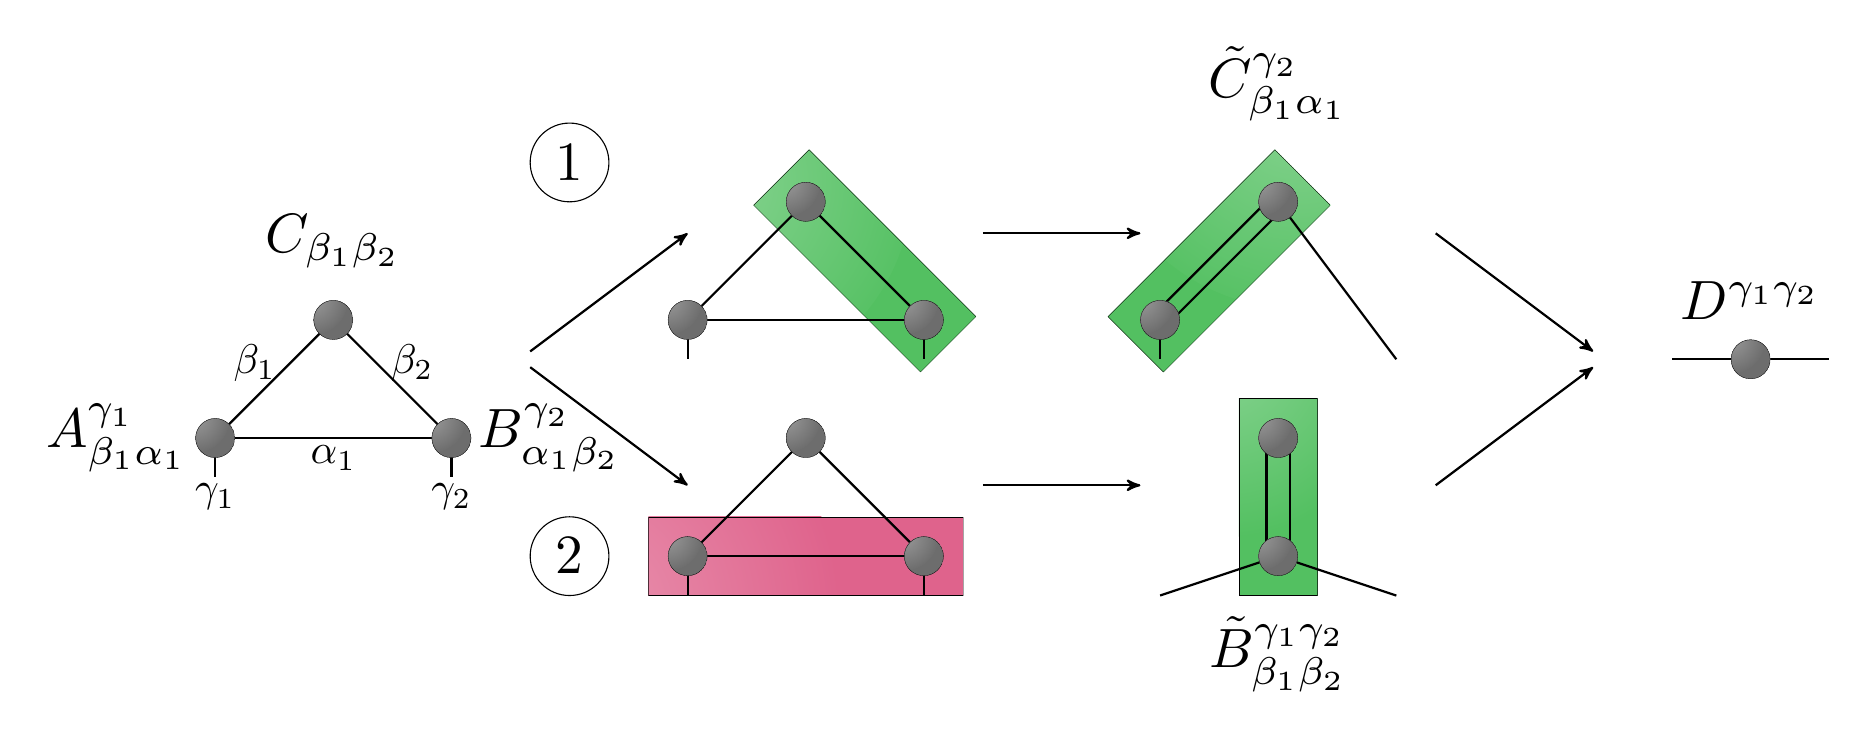
\begin{tikzpicture}
    \node (1) at (-7,-1.5) {};
    \node (2) at (-5.5,-0.0) {};
    \node (3) at (-4,-1.5) {};
    \draw [thick] (1) -- (2);
    \draw [thick] (1) -- ($(1) + (0,-0.5)$);
    \draw [thick] (1) -- (3);
    \draw [thick] (2) -- (3);
    \draw [thick] (3) -- ($(3) + (0,-0.5)$);
    \cTens{gray}{0.25}{(1)}
    \cTens{gray}{0.25}{(2)}
    \cTens{gray}{0.25}{(3)}


    \node (1) at (-1,0) {};
    \node (2) at (0.5,1.5) {};
    \node (3) at (2,0) {};
    \begin{scope}[rotate=45]
        \rTens{green}{1cm}{3cm}{($0.5*(2)+0.5*(3)$)}
    \end{scope}
    \draw[thick] (1) -- (2);
    \draw[thick] (1) -- ($(1) + (0,-0.5)$);
    \draw[thick] (1) -- (3);
    \draw[thick] (2) -- (3);
    \draw[thick] (3) -- ($(3) + (0,-0.5)$);
    \cTens{gray}{0.25}{(1)}
    \cTens{gray}{0.25}{(2)}
    \cTens{gray}{0.25}{(3)}

    \node (1) at (-1,-3) {};
    \node (2) at (0.5,-1.5) {};
    \node (3) at (2,-3) {};
    \begin{scope}[rotate=90]
        \rTens{red}{1cm}{4cm}{($0.5*(1)+0.5*(3)$)}
    \end{scope}
    \draw [thick] (1) -- (2);
    \draw [thick] (1) -- ($(1) + (0,-0.5)$);
    \draw [thick] (1) -- (3);
    \draw [thick] (2) -- (3);
    \draw [thick] (3) -- ($(3) + (0,-0.5)$);
    \cTens{gray}{0.25}{(1)}
    \cTens{gray}{0.25}{(2)}
    \cTens{gray}{0.25}{(3)}

    \node (1) at (5,0) {};
    \node (2) at (6.5,1.5) {};
    \node (3) at (8,0) {};
    \begin{scope}[rotate=-45]
        \rTens{green}{1cm}{3cm}{($0.5*(1)+0.5*(2)$)}
    \end{scope}
    \draw [thick] ($(1) + (0,0.15)$) -- ($(2) + (0,0.15)$);
    \draw [thick] ($(1) + (0,-0.15)$) -- ($(2) + (0,-0.15)$);
    \draw [thick] (1) -- ($(1) + (0,-0.5)$);
    \draw [thick] (2) -- ($(3) + (0,-0.5)$);
    \cTens{gray}{0.25}{(1)}
    \cTens{gray}{0.25}{(2)}

    \node (1) at (5,-3) {};
    \node (11) at (6.5,-3) {};
    \node (2) at (6.5,-1.5) {};
    \node (3) at (8,-3) {};
    % \shadedraw [ball color=green, rounded corners] ($(11) + (-0.5,-0.5)$) rectangle ($(2) + (0.5,0.5)$);
    \begin{scope}[rotate=0]
        \rTens{green}{1cm}{2.5cm}{($0.5*(2)+0.5*(11)$)}
    \end{scope}
    \draw [thick] ($(2) + (-0.15,0)$) -- ($(11) + (-0.15,0)$);
    \draw [thick] ($(2) + (0.15,0)$) -- ($(11) + (0.15,0)$);
    \draw [thick] (11) -- ($(1) + (0,-0.5)$);
    \draw [thick] (11) -- ($(3) + (0,-0.5)$);
    \cTens{gray}{0.25}{(11)}
    \cTens{gray}{0.25}{(2)}

    % \node (1) at (11,-1.5) {};
    \node (2) at (12.5,-0.5) {};
    % \node (3) at (14,-1.5) {};
    \draw [thick] (2) -- ++(1,0);
    \draw [thick] (2) -- ++(-1,0);
    \cTens{gray}{0.25}{(2)}

    \node[scale=2] at (6.5,-4.25) {$\tilde{B}^{\gamma_1\gamma_2}_{\beta_1\beta_2}$};
    \node[scale=2] at (8,-3) {};
    \node[scale=2] at (12.5,0.25) {$D^{\gamma_1\gamma_2}$};
    \node[scale=2] at (6.5,3) {$\tilde{C}^{\gamma_2}_{\beta_1\alpha_1}$};
    \node[scale=2] at (-8.25,-1.5) {$A^{\gamma_1}_{\beta_1\alpha_1}$};
    \node[scale=2] at (-5.5,1) {$C_{\beta_1\beta_2}$};
    \node[scale=2] at (-2.75,-1.5) {$B^{\gamma_2}_{\alpha_1\beta_2}$};
    \node[scale=1.5] at (-5.5,-1.755) {$\alpha_1$};
    \node[scale=1.5] at (-7,-2.25) {$\gamma_1$};
    \node[scale=1.5] at (-4,-2.25) {$\gamma_2$};
    \node[scale=1.5] at (-4.5,-0.55) {$\beta_2$};
    \node[scale=1.5] at (-6.5,-0.55) {$\beta_1$};
    \draw [thick, ->] (-3,-0.4)--+(2.0,1.50);
    \draw (-2.5,2) circle (0.5) node[scale=2] {$1$};
    \draw [thick, ->] (-3,-0.6)-- +(2.0,-1.50);
    \draw (-2.5,-3) circle (0.5) node[scale=2] {$2$};
    \draw [thick, ->] (2.75,-2.1)-- +(2.0,0);
    \draw [thick, ->] (2.75,1.1)-- +(2.0,0);
    \draw [thick, ->] (8.5,1.1)-- +(2.0,-1.5);
    \draw [thick, ->] (8.5,-2.1)-- +(2.0,1.5);
    % \draw [thick, ->] (2.5,1.1)--node[scale=2,above]{
    % \begin{minipage}{0.5\linewidth}
    % \begin{flalign*}
    %     \sum_{\beta_2}
    % \end{flalign*}
    % \end{minipage}}+(2.0,0.0);
    % \draw [thick, ->] (2.5,-2.1)--node[scale=2,below=-0.25cm]{
    % \begin{minipage}{0.5\linewidth}
    % \begin{flalign*}
    %     \sum_{\alpha_1}
    % \end{flalign*}
    % \end{minipage}}+(2.0,0.00);
    % \draw [thick, ->] (8,1.1)--node[scale=2,right=0.35cm,above=0.1cm]{
    % \begin{minipage}{0.5\linewidth}
    % \begin{flalign*}
    %     \sum_{\beta_1\alpha_1}
    % \end{flalign*}
    % \end{minipage}}+(2.0,-1.50);
    % \draw [thick, ->] (8,-2.1)--node[scale=2,below=0.25cm,right=-2.75cm]{
    % \begin{minipage}{0.5\linewidth}
    % \begin{flalign*}
    % \sum_{\beta_1\beta_2}
    % \end{flalign*}
    % \end{minipage}} +(2.0,+1.50);
\end{tikzpicture}


\end{document}
